\documentclass[journal]{IEEEtran}
\usepackage{lipsum} % 示例中使用的假文宏包
\ifCLASSINFOpdf
\else
   \usepackage[dvips]{graphicx}
\fi
\usepackage{url}

\hyphenation{op-tical net-works semi-conduc-tor}
\usepackage{pdfpages} % 添加pdfpages宏包
\usepackage{graphicx}
\usepackage{caption}
\usepackage{mathtools}
\usepackage{xcolor}
\usepackage{amsmath}
\usepackage{listings}
\usepackage{matlab-prettifier}
\usepackage{float}
\usepackage{subfigure}

\definecolor{matlab_comment}{RGB}{28,172,0}
\definecolor{matlab_string}{RGB}{170,55,241}
\definecolor{matlab_keyword}{RGB}{0,0,255}
\definecolor{matlab_number}{RGB}{255,255,255}

\lstset{
   backgroundcolor=\color{lightgray!20}, % 设置背景色为浅灰色
    style=Matlab-editor,
    basicstyle={\fontsize{5}{5}\ttfamily},
    keywordstyle=\color{matlab_keyword},
    commentstyle=\color{matlab_comment},
    stringstyle=\color{matlab_string},
    numberstyle=\color{matlab_number},
    numbers=left,
    numbersep=-10pt,
    showspaces=false,
    showstringspaces=false,
}
\begin{document}

\title{\color[rgb]{0,0.6,1}Digital Signal Processing Course Laboratory 7 

Digital Filter Design (December 2023)}

\author{12110405   Zhewei Chen}
%\thanks{This paragraph of the first footnote will contain the date on which you submitted your paper for review. It will also contain support information, including sponsor and financial support acknowledgment. For example, ``This work was supported in part by the U.S. Department of Commerce under Grant BS123456.'' }
%\thanks{The next few paragraphs should contain the authors' current affiliations, including current address and e-mail. For example, F. A. Author is with the National Institute of Standards and Technology, Boulder, CO 80305 USA (e-mail: author@boulder.nist.gov).}
%\thanks{S. B. Author, Jr., was with Rice University, Houston, TX 77005 USA. He is now with the Department of Physics, Colorado State University, Fort Collins, CO 80523 USA (e-mail: author@lamar.colostate.edu).}}

\markboth{EE323 Digital Signal Processing}
{Shell \MakeLowercase{\textit{et al.}}: Bare Demo of IEEEtran.cls for IEEE Journals}
\maketitle

\begin{abstract}
   This lab report will cover some basic examples of FIR and IIR filters, and then introduces the
   concepts of FIR filter design.
\end{abstract}

\begin{IEEEkeywords}
   Digital Filter, FIR Filter, IIR Filter, MATLAB
\end{IEEEkeywords}


\IEEEpeerreviewmaketitle



\section{Introduction}
\IEEEPARstart{T}{he} objective of this lab is to explore the fundamental concepts of FIR and IIR filters, their design principles, and their effects on signals (sound signals). We  will derive analytical tranfer functino, difference equation, system diagram and then use MATLAB to implement the designed filters and analyze their performance. Then we will discuss how the filter's size affects the frequency characteristics of it.




\section{Experimental Contents}
\label{sec:guidelines}


\subsection{Design of a Simple FIR Filter}



Analytical transfer function:
\[
H_{f}(z) = (1 - z_{1}z^{-1})(1 - z_{2}z^{-1})
\]
\[
= (1 - e^{j\theta}z^{-1})(1 - e^{-j\theta}z^{-1})
= 1 - 2z^{-1}\cos \theta + z^{-2}
\]
Impulse response:
\[h_{f}[n] = \delta[n] - 2 \delta[n-1] \cos \theta + \delta[n-2]\]
Difference equation:
\[y[n] = x[n] - 2 x[n-1] \cos \theta + x[n-2]\]
The system diagram:
\begin{figure}[htbp]
   \centering
   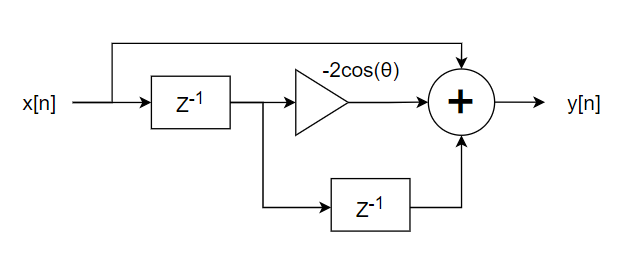
\includegraphics[width=0.42\textwidth]{2.png} 
\caption{The System Diagram of FIR Filter \(H_f\) }
 \end{figure}

 Using MATLAB to research how \(\theta\) affects the magnitude response of \(H_f\) :
 \begin{lstlisting}[style=Matlab-editor]
   w=-pi:0.01:pi;
   z=exp(1i*w);
   H1=1-2*cos(pi/6)*z.^(-1)+z.^(-2);
   H2=1-2*cos(pi/3)*z.^(-1)+z.^(-2);
   H3=1-2*cos(pi/2)*z.^(-1)+z.^(-2);
\end{lstlisting}

\begin{figure}[htbp]
   \centering
   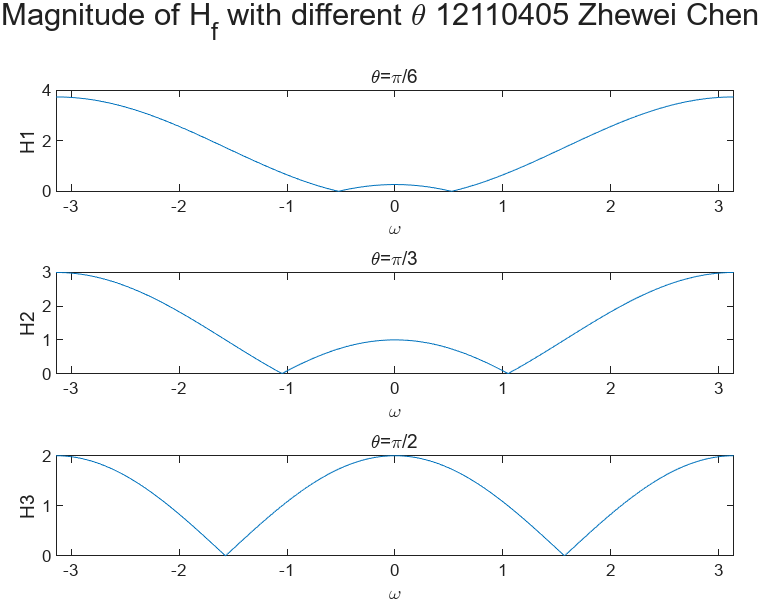
\includegraphics[width=0.5\textwidth]{31.png} 
\caption{Plot of \(\lvert H_{f}\rvert\) with different \(\theta\)}
 \end{figure}

\textcolor[rgb]{0,0.6,1}{Analysis:}

\textcolor[rgb]{0,0.6,1}{-}The frequency response shows that it is a bandstop filter.

\textcolor[rgb]{0,0.6,1}{-}When \( \omega=\theta \),  \(|H_f(e^{j\omega})|=0\),which shows \( \omega=\theta \) is the center frequency of this bandstop filter.
When \(\theta\) decreases(increases), the center frequency of the bandstop filter decreases(increases).


Then we write a Matlab function \(\mathbf{FIRfilter(x)}\) that implements the filter \(H_f(z)\) with the measured value of \(\theta\) and outputs the filtered signal.

 \begin{lstlisting}[title={FIRfilter.m},style=Matlab-editor]
   function y = FIRfilter(x)
   [X,w]=DTFT(x,0);
   [~,Imax]=max(abs(X));
   h=[1 -2*cos(w(Imax)) 1];
   y=conv(x,h);
   end   
\end{lstlisting}

And applying the \(\mathbf{nspeech1} \) vector to attenuate the sinusoidal interference. 

 \begin{figure}[H]
   \centering
   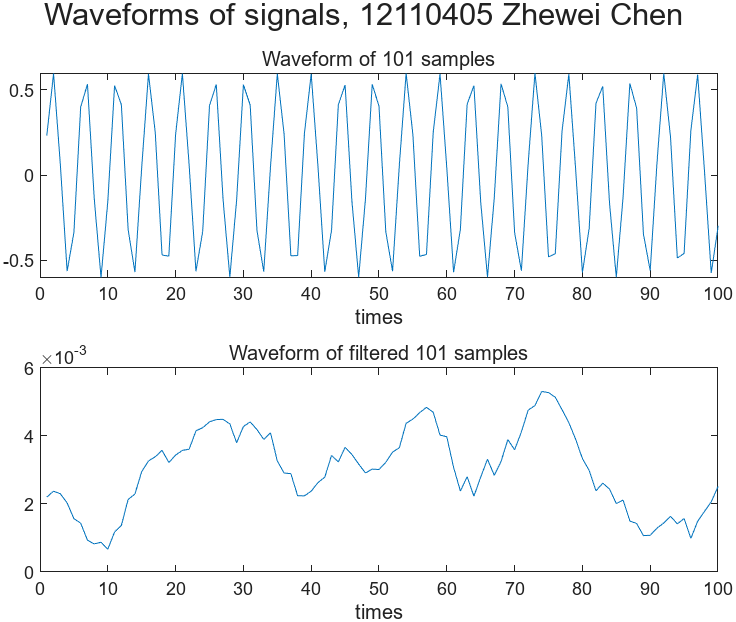
\includegraphics[width=0.42\textwidth]{33.png} % 将"your_image.png"替换为您的PNG图片文件名
\caption{Plot of Waveforms of 101 Samples of Signal and Filtered Signal}
 \end{figure}

 \textcolor[rgb]{0,0.6,1}{Analysis:}


 \textcolor[rgb]{0,0.6,1}{-}The original signal approximates a sine wave.

 \textcolor[rgb]{0,0.6,1}{-}The filtered signal has a lower volume than the orignal signal.

 \begin{figure}[H]
   \centering
   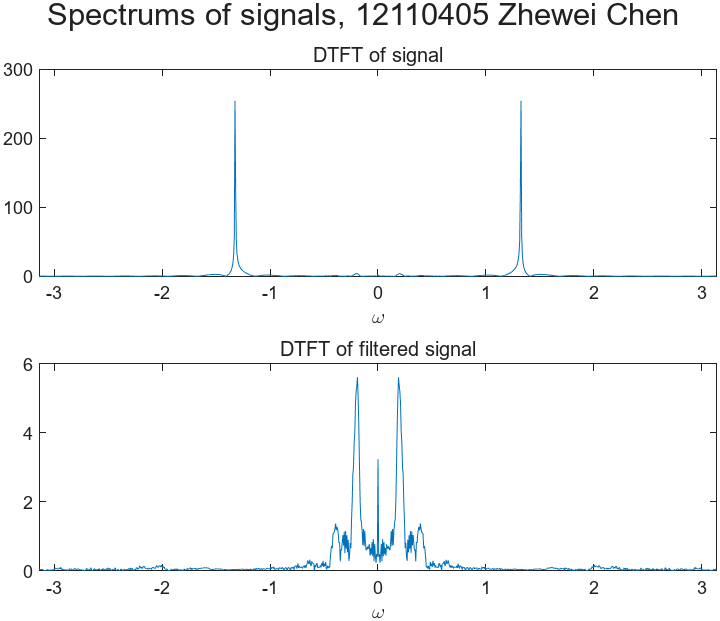
\includegraphics[width=0.4\textwidth]{32.png} % 将"your_image.png"替换为您的PNG图片文件名
\caption{Spectrums of DTFTs of Signal and Filtered Signal}
 \end{figure}


 \textcolor[rgb]{0,0.6,1}{Analysis:}


\textcolor[rgb]{0,0.6,1}{-}This is a bandstop filter.

\textcolor[rgb]{0,0.6,1}{-}The noise of the orignal signal has been filtered, we can hear the voice more clearly.





\subsection{Design of a Simple IIR Filter}

Analytical transfer function:
\[
H_i(z)=\frac{1-r}{1-2r\cos\theta z^{-1}+r^2z^{-2}}
\]

Impulse response:
\[h_{i}[n] = \frac{(1-r)\delta [n]}{\delta [n]-2r\delta [n-1] \cos \theta +r^{2} \delta [n-2]}\]
Difference equation:
\[y[n]-2 r \cos \theta y[n-1]+r^{2} y[n-2]=(1-r) x[n]\]
The system diagram:

\begin{figure}[H]
   \centering
   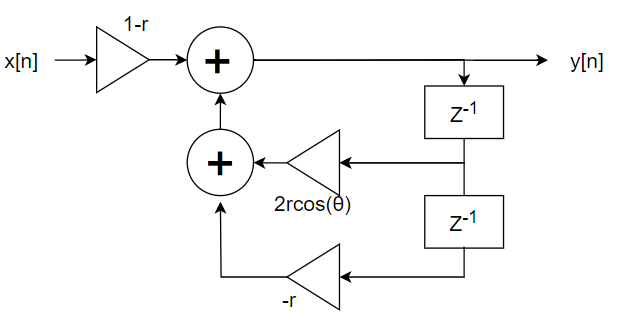
\includegraphics[width=0.35\textwidth]{1.png} % 将"your_image.png"替换为您的PNG图片文件名
\caption{The System Diagram of IIR Filter \(H_i\)}
 \end{figure}

Using MATLAB to research how \(r\) affects the magnitude response of \(H_i\) :


\begin{lstlisting}[style=Matlab-editor]
   w1=-pi:0.01:pi;
   z=exp(1i*w1);
   r1=0.99;
   r2=0.9;
   r3=0.7;
   H1=(1-r1)./(1-2*r1*cos(pi/3).*z.^(-1)+r1.^2.*z.^(-2));
   H2=(1-r2)./(1-2*r2*cos(pi/3).*z.^(-1)+r2.^2.*z.^(-2));
   H3=(1-r3)./(1-2*r3*cos(pi/3).*z.^(-1)+r3.^2.*z.^(-2));
\end{lstlisting}


\begin{figure}[htbp]
   \centering
   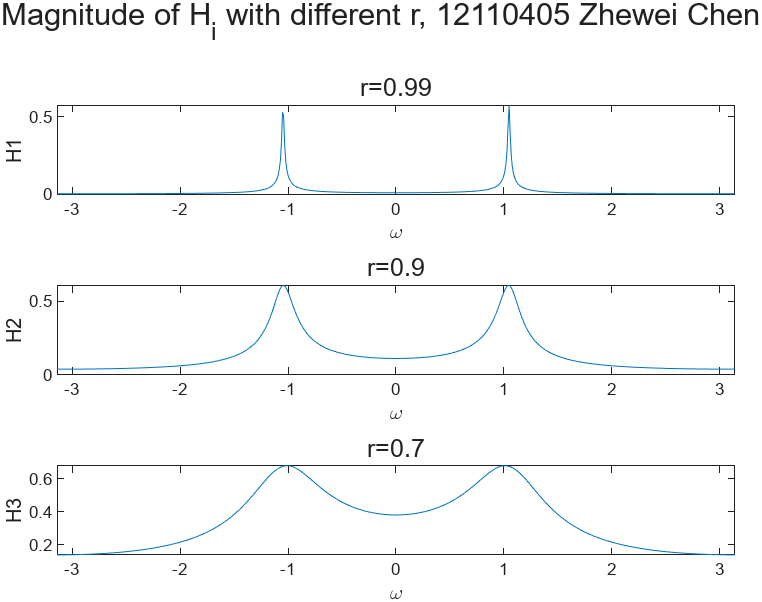
\includegraphics[width=0.4\textwidth]{41.png} % 将"your_image.png"替换为您的PNG图片文件名
\caption{Plot of \(\lvert H_{i}\rvert\) with different \(r\)}
 \end{figure}

\textcolor[rgb]{0,0.6,1}{Analysis:}

As r increases, the magnitude responses will be more sharp, and similar to a bandpass filter.

Write a Matlab function \(\mathbf{ IIRfilter.m }\) that implements the filter \(H_i(z)\).

\begin{lstlisting}[title={IIRfilter.m},style=Matlab-editor]
   function y = IIRfilter(x)
   theta=(3146/8000)*2*pi;
   r=0.995;
   N=length(x);
   y=zeros(1,N);
   y(1)=(1-r)*x(1);
   y(2)=(1-r)*x(2)+2*r*cos(theta)*y(1);
   for k=3:N
       y(k)=(1-r)*x(k)+2*r*cos(theta)*y(k-1)-r^2*y(k-2);
    end
   end    
\end{lstlisting}

\begin{figure}[htbp]
   \centering
   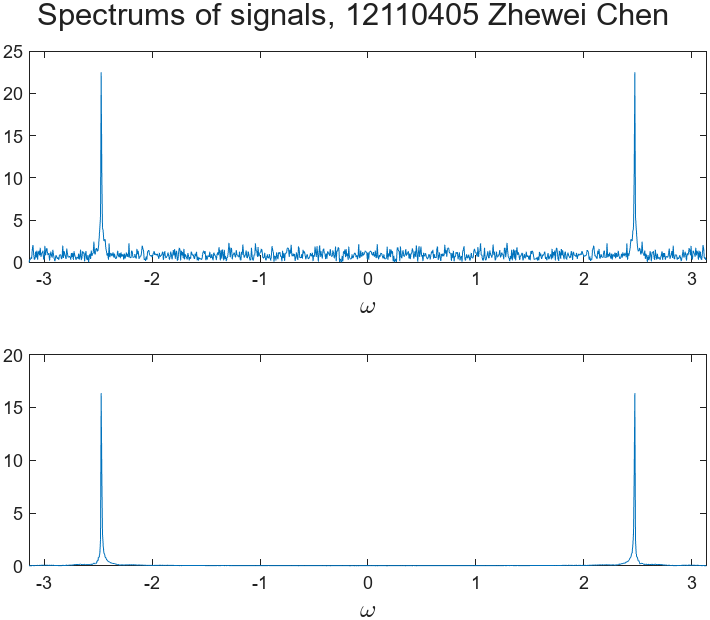
\includegraphics[width=0.4\textwidth]{42.png}
\caption{Plot of Spectrums of Signals and Filtered Signals}
   \end{figure}
   
\begin{figure}[htbp]
   \centering
   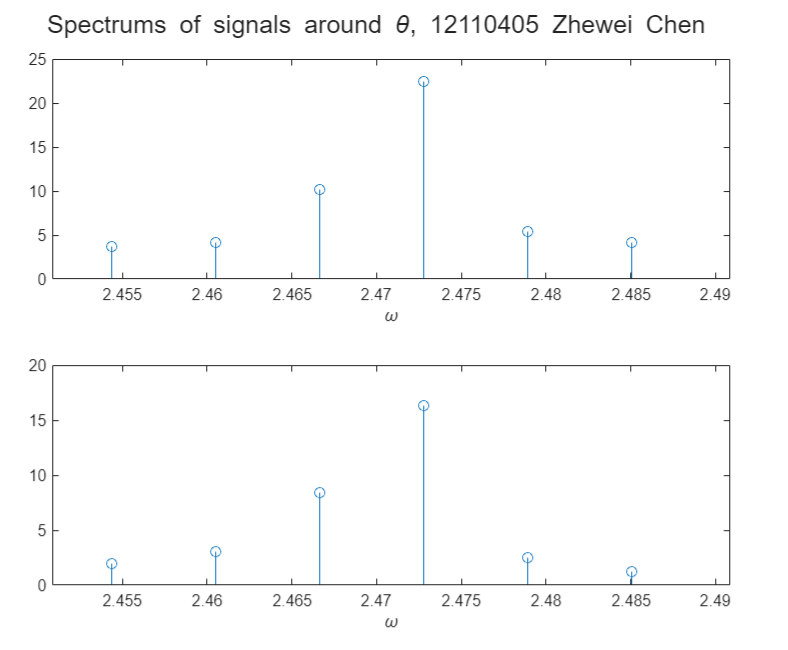
\includegraphics[width=0.4\textwidth]{43.png}
\caption{Plot of Spectrums of Signals Around \(\theta\)}
   \end{figure}

   \begin{figure}[htbp]
      \centering
      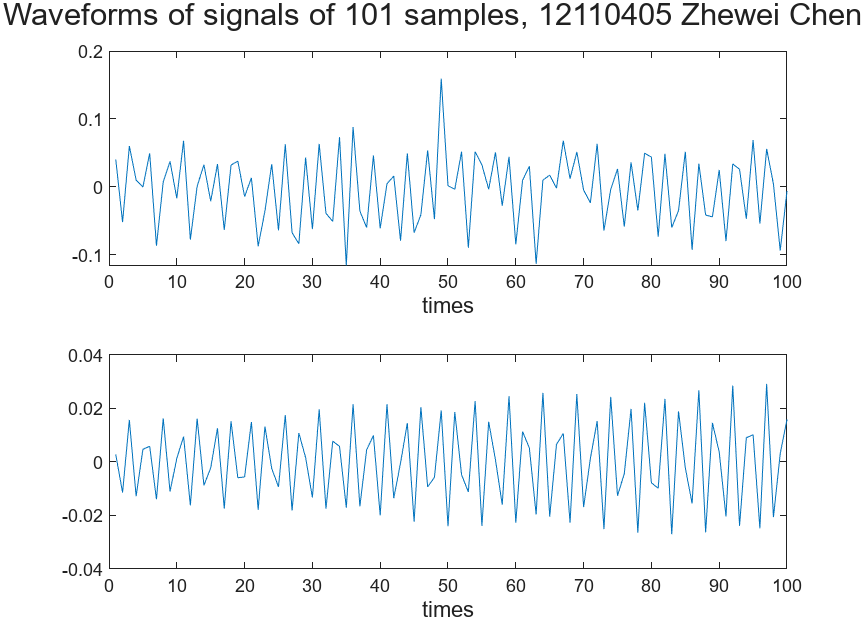
\includegraphics[width=0.43\textwidth]{44.png}
   \caption{Plot of Waveforms of 101 Samples}
      \end{figure}

\textcolor[rgb]{0,0.6,1}{Analysis:}

\textcolor[rgb]{0,0.6,1}{-}The magnitude of frequency that is not around \(\theta \) in the frequency domain decreases a lot after filtering.

\textcolor[rgb]{0,0.6,1}{-}The spectrums show that the magnitude of DTFT of signal decreases a bit after filtering  around \(\theta\)

\textcolor[rgb]{0,0.6,1}{-}The volume decreases a bit after filtering but we can hear more clearly.



\begin{figure}[htbp]
   \centering
   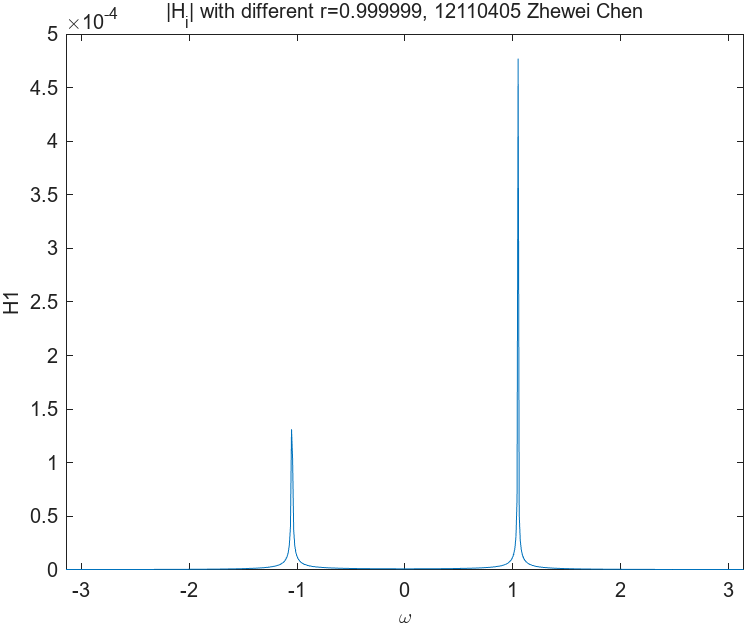
\includegraphics[width=0.3\textwidth]{40.png}
\caption{Plot of \(\lvert H_{i}\rvert\) with \(r\)=0.999999}
   \end{figure}

\textcolor[rgb]{0,0.6,1}{Analysis:}

\textcolor[rgb]{0,0.6,1}{-}When r=0.999999 (very close to 1), we can hear nothing.Because the magnitude response shows that the volume of the signal decrease to much.Though it is still a bandpass filter. 

\subsection{Filter Design Using Truncation}
To examine the effect of filter size on the frequency characteristics of the filter, write a Matlab 
function \(\mathbf{LPFtrunc.m}\) that computes the truncated and shifted impulse response of size 𝑁 for a 
lowpass filter with a cutoff frequency of \(\omega_c\) = 2.0.
\begin{lstlisting}[title={LPFtrunc.m},style=Matlab-editor]
   function h = LPFtrunc(N)
   n=0:N-1;
    h = 2/pi * sinc(2/pi * ( n - (N-1)/2));
   end   
\end{lstlisting}

\textcolor[rgb]{0,0.6,1}{Analysis:}

\textcolor[rgb]{0,0.6,1}{-}We can use matrix multiplication to aviod the for loop.


\begin{figure}[H]
   \centering
   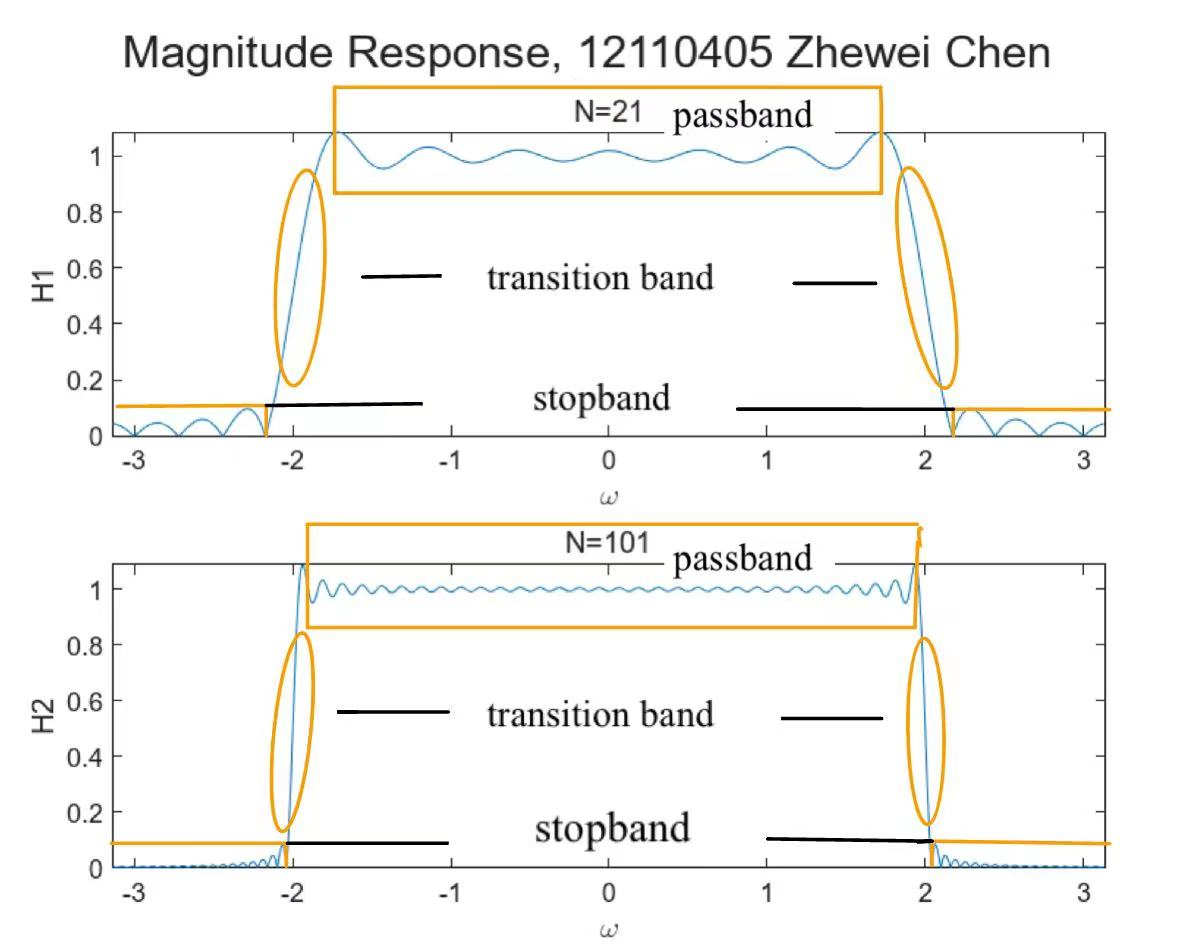
\includegraphics[width=0.35\textwidth]{61.png}
\caption{Plot of Magnitude Response N = 101 and N = 21}
   \end{figure}




\begin{figure}[htbp]
   \centering
   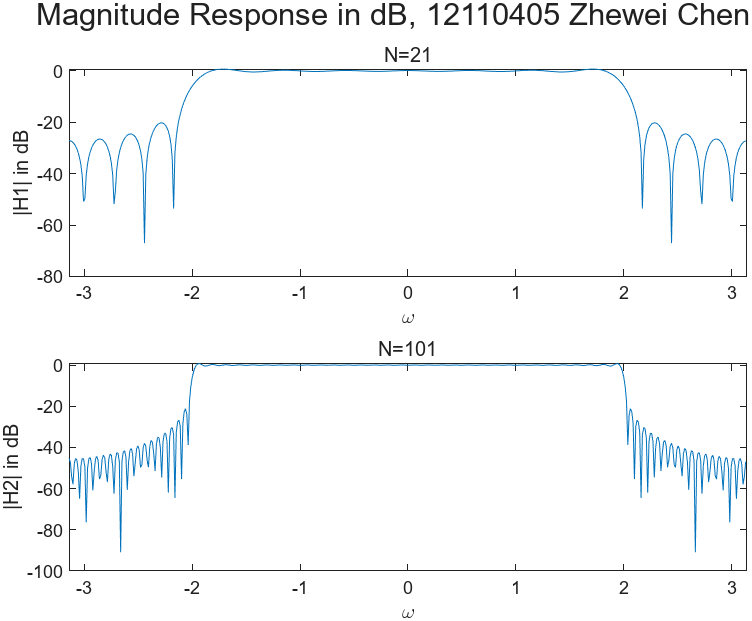
\includegraphics[width=0.4\textwidth]{62.png}
\caption{Plot of Magnitude Response in dB N = 101 and N = 21}
   \end{figure}

\textcolor[rgb]{0,0.6,1}{Analysis:}

\textcolor[rgb]{0,0.6,1}{-}
Clearly we can observe the Gibbs Phenomenon.
When N increases, the influence of Gibbs Phenomenon decreases and the filtering becomes more similar to a ideal lowpass filter because of the more sampling points.

\begin{figure}[htbp]
   \centering
   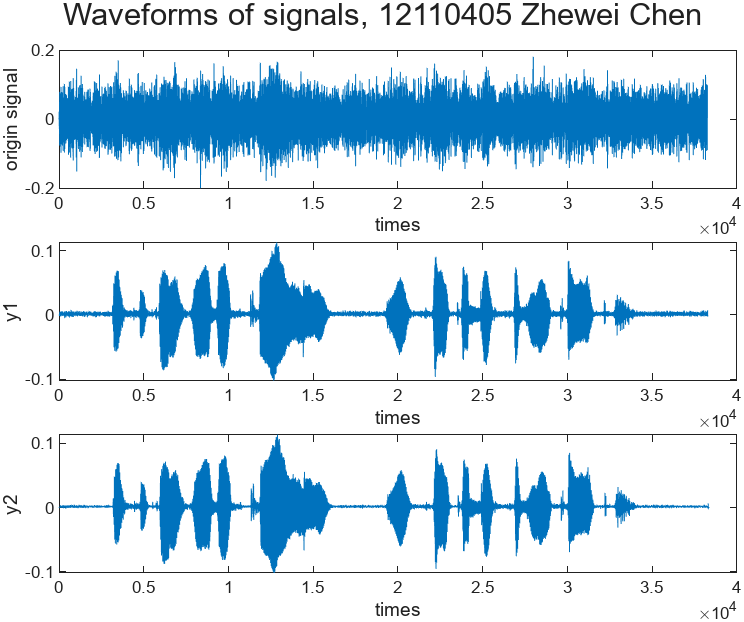
\includegraphics[width=0.4\textwidth]{63.png}
\caption{Plot of Waveforms of Signal and Filtered Signals}
   \end{figure}      

\textcolor[rgb]{0,0.6,1}{Analysis:}

\textcolor[rgb]{0,0.6,1}{-}After hear and observing the waveforms of sound and filtered sound.We observe that \(y_2\), which is filtered by the truncated impulse response of size 101, contains \(\mathbf{less~noise}\)  than \(y_1\), which is filtered by the truncated impulse response of size 21.











\section{Conclusion}
Through this experiment, we attempted to derive the theoretical forms of filter design, including difference equations and system diagrams, using mathematical methods. We then implemented these designs using MATLAB. By observing the spectrum, waveform, and listening to the filtered signals, we studied the characteristics of the signals before and after filtering. Constantly adjusting parameters allowed for comprehensive and detailed exploration of the results.

During the experiment, we also discovered the limitations of simple filters. When the filtering effect was significant, there was often a considerable loss in volume. This highlighted the need for alternative methods to compensate for the volume loss and overcome the limitations of simple filters.

\end{document}
